\FloatBarrier
\section{Methodology}
\label{sec:methodology}

This section describes the model architectures and the training protocol for the
experiments in this thesis, together with the reasoning behind the design choices.
The experiments share a common discipline. Since it proved too difficult to train a purely quantum model on raw spectra, every quantum model in this thesis is hybrid, a classical feature extractor followed by a small variational quantum circuit. Each is benchmarked against a classical counterpart built to the same shape and trained
under an identical protocol, so that an observed difference can be attributed to the
contested component. Where the experiments differ is in the feature stage.
We have experimented with a vast range of architectures and training protocols, and the ones described here are the ones that worked best.
They are not the only ones we tried, and they are not necessarily the best possible, but they are the ones that we settled on after a long process of trial and error. The full implementation is released as a reproducibility package.\footnote{\url{https://github.com/ShpetimV/QML-AnalyzingGalaxies}}


\subsection{Experiment 3: Classifier Heads on a Frozen Extractor}
\label{sec:exp3_methods}

\subsubsection{Design Principles}
\label{sec:exp3_philosophy}

The design of Experiment 3 follows two principles, control and fairness. Control,
because we want every measured difference to come from a single place. By reusing a
strong pretrained network as a frozen feature extractor and varying only the small
head on top of it, we remove feature learning from the comparison and reduce it to a
question about the head alone. Fairness, because a quantum head and a classical head
cannot be compared simply by counting parameters, since a quantum rotation angle and
a classical weight are not equivalent units of capacity. Rather than equate units we
hold the architecture fixed and swap only the internals of the head, building a
classical control with exactly the same parameter count and pipeline shape as the
quantum model. A third principle, prompted by supervisor feedback, is that the
parameter count alone is too narrow a lens, so we also examine convergence speed,
training stability and computational cost rather than final accuracy alone. The four
heads introduced below are the instruments through which these principles are
applied.

\subsubsection{Frozen Feature Extractor (the Beast)}
\label{sec:beast}

The shared backbone is a pretrained one-dimensional classifier that we refer to as
the Beast. It combines a multi-scale convolutional stem, squeeze-and-excitation
residual blocks and a two-layer Transformer encoder, totalling about 14 million
parameters, and was trained from scratch on the full 62-class problem where it
reaches roughly 84\% accuracy. For Experiment 3 its final
\texttt{Linear(128, num\_classes)} layer is replaced by an identity map and every
parameter is frozen, so the backbone becomes a fixed function that turns each
spectrum into the same 128-dimensional feature vector. We freeze it rather than
fine-tune it for two reasons. First, a 14-million-parameter backbone trained jointly
with a tiny head could absorb or mask the behaviour of that head and confound the
comparison, whereas a fixed backbone presents every head with identical inputs.
Second, simulating the quantum circuit is expensive, and reusing a pretrained
extractor avoids repeatedly backpropagating through both the backbone and the
circuit. The backbone is also kept permanently in evaluation mode so that its
batch-normalisation running statistics do not drift while the head is trained.

\subsubsection{Classification Heads}
\label{sec:heads}

Every head maps the 128-dimensional features to four class logits. Four heads are
compared, and they are chosen so that each isolates a specific question.

The \emph{dense classical head} (Model~A) is a two-layer perceptron,
\texttt{Linear(128,38)} $\to$ ReLU $\to$ Dropout$(0.2)$ $\to$ \texttt{Linear(38,4)},
with $128\cdot 38 + 38 = 4902$ and $38\cdot 4 + 4 = 156$ weights, for $5058$
trainable parameters. It is the conventional, comfortably sized baseline and answers
the question of what accuracy is reachable when the head is not parameter-starved.
Its full pipeline, the frozen extractor followed by the two-layer head, is shown in
Figure~\ref{fig:densehead}.

\begin{figure*}[t]
\centering
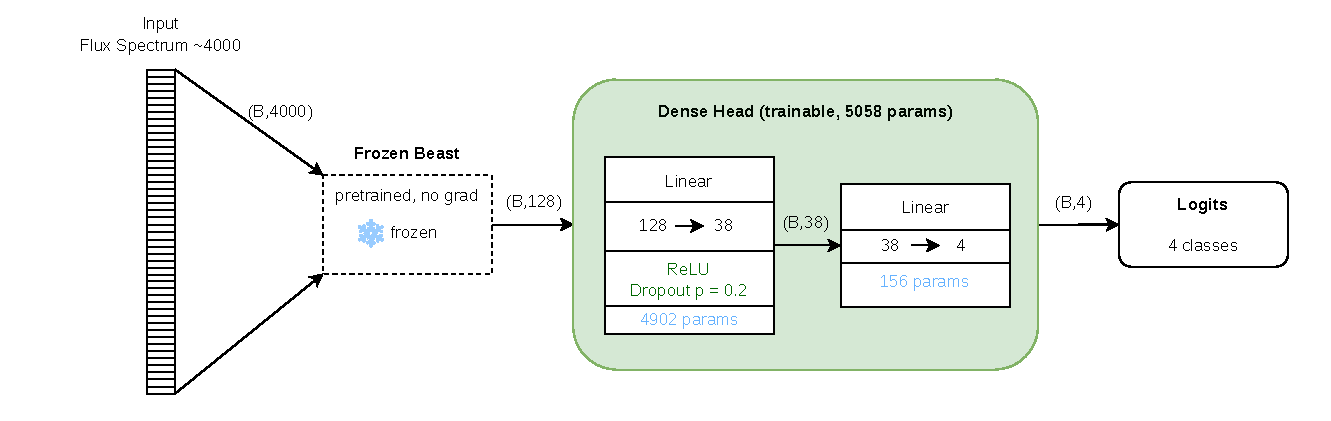
\includegraphics[width=\textwidth]{Figures/dense_head.pdf}
\caption{Complete data flow of the dense classical head (Model~A). The frozen Beast
maps the input flux spectrum to a 128-dimensional feature vector, which the trainable
two-layer head turns into class logits through \texttt{Linear(128,38)}, a ReLU and
dropout, and \texttt{Linear(38,4)}, for $5058$ trainable parameters. This is the only
head that does not pass through a four-dimensional bottleneck.}
\label{fig:densehead}
\end{figure*}

The \emph{hybrid quantum head} (Model~B) first compresses the features with a
trainable \texttt{Linear(128,4)} bottleneck of $516$ parameters, squashes the four
outputs into $[-\pi,\pi]$ with a $\tanh(\cdot)\,\pi$ transform and feeds them to the
variational quantum circuit of Section~\ref{sec:vqc} and Figure~\ref{fig:vqc}. The
four Pauli-$Z$ expectations returned by the circuit pass through a trainable
\texttt{Linear(4,4)} readout of $20$ parameters, which with the $20$ circuit angles
gives $556$ trainable parameters. Two choices in this head are deliberate. The
bottleneck is trainable rather than fixed because the circuit accepts only four
numbers, and gradient descent can then discover the four discriminative directions
the circuit needs instead of being handed an arbitrary projection. The readout is a
trainable linear layer because the raw expectation values are confined to $[-1,1]$
and tie qubit $i$ to class $i$, so passing them through a learned map lets the logits
leave that range and removes the artificial cap on softmax confidence. The complete
pipeline of this head, from the input spectrum through to the class logits, is shown
in Figure~\ref{fig:modelb}.

The \emph{parameter-matched classical controls} (Models~C and~D) are the embodiment
of the fairness principle. They are structural mirrors of the hybrid head in which
the quantum circuit is replaced by a classical block of exactly the same parameter
count. Both use a \texttt{Linear(128,4)} bottleneck followed by a $\tanh$, which
reproduces the bounded input that the circuit receives, then a middle
\texttt{Linear(4,4)} that stands in for the circuit and a \texttt{Linear(4,4)}
readout, again $516 + 20 + 20 = 556$ trainable parameters. Matching the count by
construction sidesteps the objection that an angle and a weight are not comparable
units. Model~C places a ReLU between the two width-4 layers and Model~D places a
$\tanh$ there instead. This single controlled change exists to test whether any
behaviour attributed to the quantum circuit might instead be an optimisation artefact
of the surrounding classical structure, a question taken up in the results. The three
interchangeable middle stages that distinguish Models~B, C and~D are compared in
Figure~\ref{fig:middles}, with every other stage of the pipeline in
Figure~\ref{fig:modelb} held identical.

\begin{figure}[t]
\centering
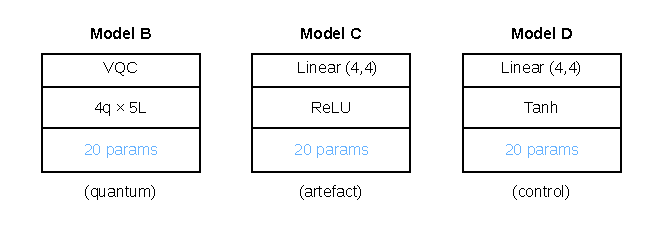
\includegraphics[width=\columnwidth]{Figures/3models.pdf}
\caption{The three interchangeable middle stages that distinguish Models~B, C and~D.
Each is a 20-parameter block occupying the same slot in the otherwise identical
pipeline of Figure~\ref{fig:modelb}. Model~B uses the variational quantum circuit,
whereas Models~C and~D replace it with a classical \texttt{Linear(4,4)} layer under a
ReLU or a $\tanh$ activation. Holding every other stage fixed isolates the effect of
this single block.}
\label{fig:middles}
\end{figure}

\begin{figure*}[t]
\centering
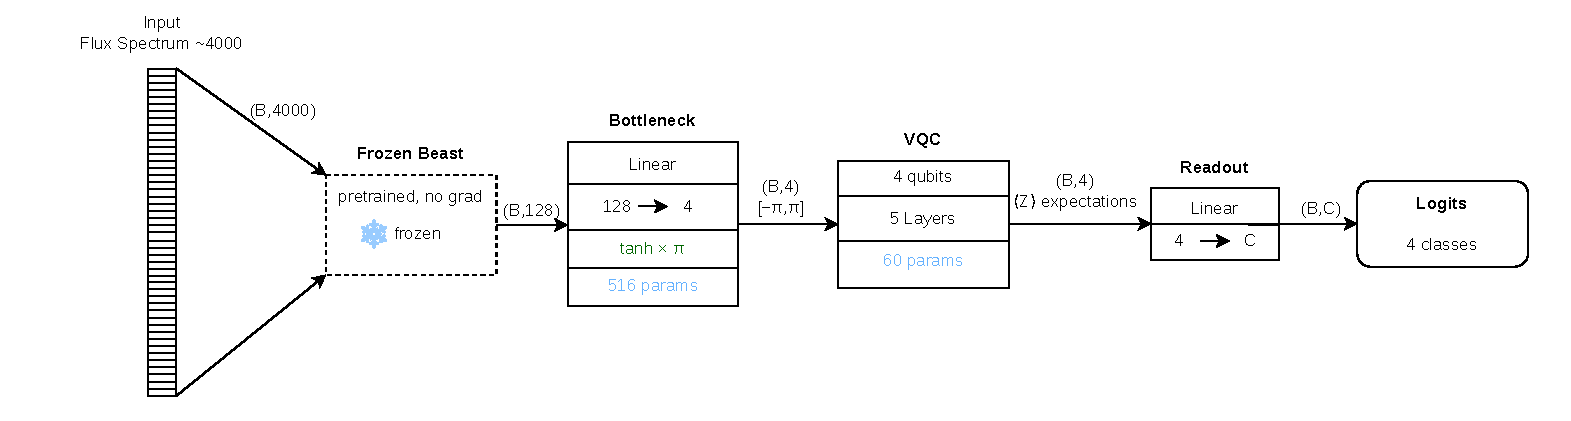
\includegraphics[width=\textwidth]{Figures/model_b_complete.pdf}
\caption{Complete data flow of the hybrid quantum head (Model~B). The input flux
spectrum is mapped by the frozen Beast to a 128-dimensional feature vector,
compressed by the trainable \texttt{Linear(128,4)} bottleneck and squashed into
$[-\pi,\pi]$ by a $\tanh(\cdot)\,\pi$ transform, processed by the four-qubit
variational quantum circuit (detailed in Figure~\ref{fig:vqc}) whose four
Pauli-$Z$ expectations are turned into class logits by the trainable
\texttt{Linear(4,$C$)} readout. Tensor shapes are given along the arrows for a
batch of size $B$ and $C=4$ classes.}
\label{fig:modelb}
\end{figure*}

\subsubsection{Variational Quantum Circuit}
\label{sec:vqc}

The quantum head maps the four real values produced by the trainable bottleneck into
the circuit shown in Figure~\ref{fig:vqc}. The four numbers, already squashed into
$[-\pi,\pi]$, are used as rotation angles. Each layer re-uploads these inputs with
$R_Y$ rotations, applies a trainable $R_Y(\theta^{(\ell)}_q)$ rotation on every qubit
and entangles the register with a ring of CNOT gates. After $L=5$ layers each qubit
is measured in the Pauli-$Z$ basis, and the four expectation values feed the
trainable readout. Three of these choices reflect a preference for the smallest
circuit that can still express the task. Data re-uploading, the re-injection of the
input in every layer, lets a shallow circuit represent higher-order functions of its
input that a single encoding layer cannot reach. Single-axis $R_Y$ rotations keep the
budget at one trainable angle per qubit per layer, and an exploratory variant with
full three-axis rotations added parameters without improving accuracy. The ring of
CNOT gates is a simple, hardware-friendly entangler that spreads correlations across
all four qubits at a depth that grows only linearly with their number.

\begin{figure}[t]
\centering
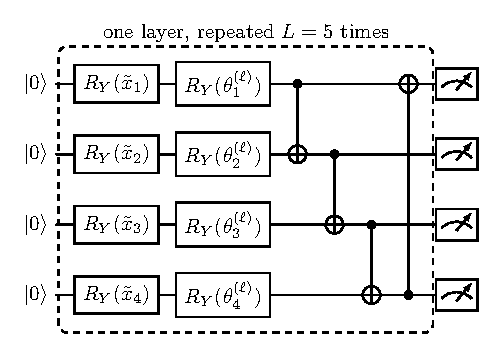
\includegraphics[width=\columnwidth]{Figures/vqc_circuit.pdf}
\caption{Variational quantum circuit of the quantum head (Model~B). The four qubits
start in $|0\rangle$. Within each layer the bottleneck outputs $x_q$ are re-uploaded
through $R_Y(x_q)$ rotations, followed by trainable $R_Y(\theta^{(\ell)}_q)$
rotations and a ring of CNOT gates. The dashed block is repeated $L=5$ times. A
final Pauli-$Z$ measurement on each qubit yields four expectation values that are
passed to a trainable linear readout. The $20$ trainable circuit angles are the
$\theta^{(\ell)}_q$ for $\ell=1,\dots,5$ and $q=1,\dots,4$.}
\label{fig:vqc}
\end{figure}

\subsubsection{Encoding Variants for the Ablation}
\label{sec:encoding}

The trainable bottleneck of Model~B couples two things that we would like to separate,
the number of qubits and the way features are loaded into them. To tell them apart we
replace the learned bottleneck with frozen alternatives that change only the encoding.
A \texttt{FrozenPCABottleneck} fits a principal-component projection once on the
training-set features and then keeps it fixed, so it is informative but not learnable.
The \emph{pure-PCA} variant feeds a frozen \texttt{PCA(128,4)} directly into the same
circuit and readout, leaving only the $20$ circuit angles and the $20$ readout weights
trainable, about $40$ parameters in total. A \emph{PCA-hybrid} variant inserts a small
trainable \texttt{Linear(64,4)} after a frozen \texttt{PCA(128,64)}, for roughly $300$
trainable parameters. Both are compared against the learned \texttt{Linear(128,4)} of
Model~B, which encodes into the same four qubits but chooses its directions
end-to-end through the loss. Because the qubit count is held at four throughout, any
difference between these variants must come from the encoding rather than from the
size of the circuit.

\subsubsection{Training Protocol}
\label{sec:training}

Experiment 3 uses a four-class subset balanced to 1000 samples per class and split
$70/15/15$ into train, validation and test with seed $42$. All heads are trained on
top of the frozen extractor with the Adam optimiser at a learning rate of $10^{-3}$
and weight decay $10^{-4}$, a batch size of $256$ and a cross-entropy loss, for 100
epochs. The PCA-based variants fit their projection on the training features once
before optimisation begins. The extractor remains frozen and in evaluation mode
throughout. In line with the design principles we record not only the final test
accuracy but also per-class recall, the test confusion matrices, the convergence
behaviour and the training cost.
